% =============================================================================
%  From Lecture Materials to Structured Educational Content
%  Design and Implementation of an AI-Assisted Learning Platform
%
%  Bachelor thesis — Informatik
%
%  BUILD:  make          (builds figures, then the document, via latexmk)
%          make quick    (single pdflatex pass, no bibliography — fast preview)
%
%  REPARENTING FOR A UNIVERSITY TEMPLATE
%  Almost every institute supplies its own class or style file. This skeleton is
%  deliberately shallow so that swap is cheap: the class is chosen on the next
%  line, all packages live in preamble.tex, and all title-page data lives in
%  metadata.tex. Chapter files under chapters/ contain no formatting decisions,
%  so they drop into a different template unchanged.
% =============================================================================

% scrreprt (KOMA-Script) is the common choice for German university theses.
% Replace this single line if your institute mandates a class.
\documentclass[
  a4paper,
  11pt,
  twoside,          % printed and bound: different margins on odd/even pages
  openright,        % chapters start on a right-hand page
  numbers=noenddot,
  listof=totoc,
  bibliography=totoc,
  english,
]{scrreprt}

% =============================================================================
%  Packages and document-wide settings.
%
%  Kept separate from main.tex so a university template can replace the class
%  and title page without touching this file, or replace this file wholesale
%  without touching any chapter.
% =============================================================================

% --- Encoding and language ----------------------------------------------------
\usepackage[T1]{fontenc}
\usepackage[utf8]{inputenc}
\usepackage[english]{babel}
\usepackage{csquotes}          % required by biblatex; also gives \enquote{}
\usepackage{microtype}         % subtle spacing/protrusion — noticeably better justification

% --- Maths --------------------------------------------------------------------
\usepackage{amsmath}
\usepackage{amssymb}

% --- Figures and tables -------------------------------------------------------
\usepackage{graphicx}
\graphicspath{{figures/}}      % so 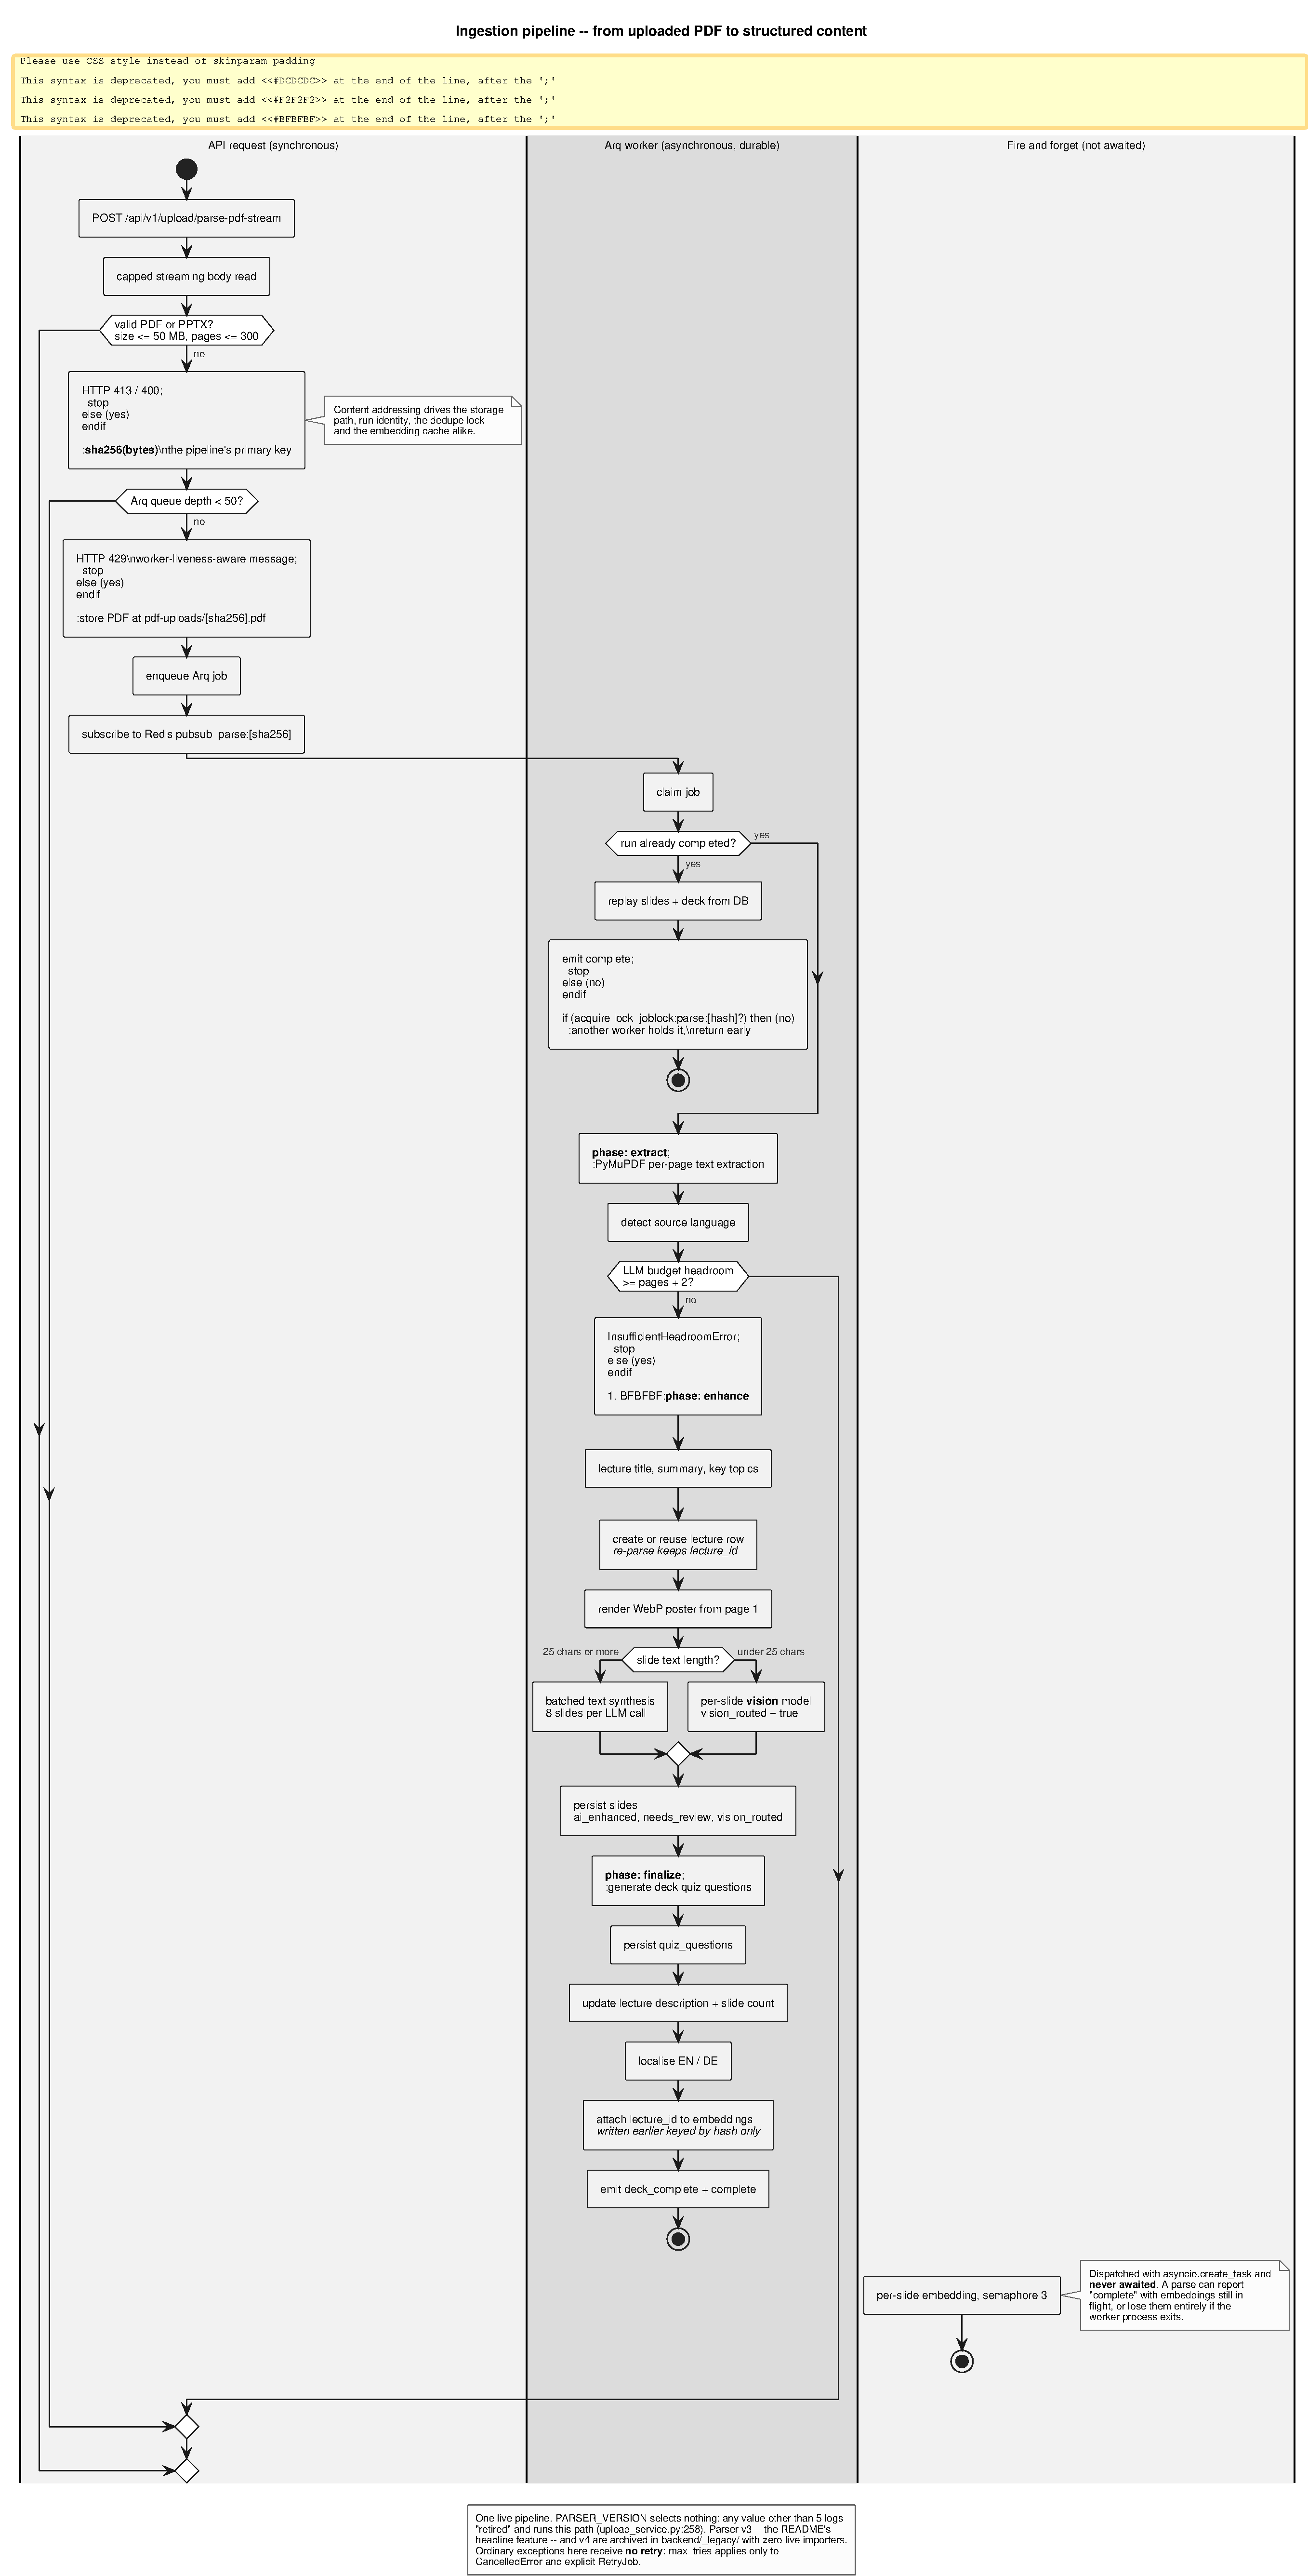
\includegraphics{f8-pipeline} just works
\usepackage{booktabs}          % \toprule/\midrule/\bottomrule — no vertical rules
\usepackage{longtable}         % tables that span pages (the honesty ledger will)
\usepackage{float}
\usepackage[export]{adjustbox} % lets a too-wide figure be scaled in place

% IMPORTANT — PDF 2.0 figure inclusion.
% The PlantUML-generated figures are PDF 2.0. pdfTeX refuses to \includegraphics
% a PDF whose version exceeds its own output version, failing with
%   "PDF inclusion: found PDF version <2.0>, but at most version <1.7> allowed".
% Raising the output version fixes it on TeX Live 2023+. \pdfvariable is
% undefined on older engines, hence the guard.
%
% If you still hit that error, switch the figure pipeline to EPS: set
%   PDF_FLAG = -teps
% in figures/Makefile and add an epstopdf step (epstopdf ships with TeX Live).
\ifdefined\pdfvariable
  \pdfvariable majorversion=2
  \pdfvariable minorversion=0
\fi

% --- Code listings ------------------------------------------------------------
\usepackage{listings}
\lstset{
  basicstyle=\ttfamily\footnotesize,
  breaklines=true,
  captionpos=b,
  frame=single,
  showstringspaces=false,
  numbers=left,
  numberstyle=\tiny\color{gray},
  keywordstyle=\bfseries,
  commentstyle=\itshape\color{gray},
  columns=fullflexible,
}
\usepackage{xcolor}

% --- Bibliography -------------------------------------------------------------
% numeric-comp compresses [1,2,3] into [1-3]. Swap style= if your institute
% mandates author-year (e.g. style=authoryear).
\usepackage[
  backend=biber,
  style=numeric-comp,
  sorting=nyt,
  maxbibnames=99,
  giveninits=true,
]{biblatex}
\addbibresource{references.bib}

% --- Cross-references (load hyperref late, cleveref last) ---------------------
\usepackage[
  hidelinks,                   % no coloured boxes — correct for a printed thesis
  pdfusetitle,
]{hyperref}
\usepackage[capitalise,noabbrev]{cleveref}

% --- Convenience --------------------------------------------------------------

% Standard figure inclusion. Usage:
%   \thesisfigure{f8-pipeline}{Ingestion pipeline, five observable phases.}{fig:pipeline}
% The figures are tall and narrow or wide and short depending on type, so width
% is capped at \textwidth and height at 0.85\textheight; whichever binds first
% wins, and nothing overflows the page.
\newcommand{\thesisfigure}[3]{%
  \begin{figure}[htbp]
    \centering
    \includegraphics[width=\textwidth,height=0.85\textheight,keepaspectratio]{#1}%
    \caption{#2}%
    \label{#3}%
  \end{figure}%
}

% Same, but for a figure that needs a full page of its own (the ER diagram and
% the tutor sequence diagram will).
\newcommand{\thesisfigurepage}[3]{%
  \begin{figure}[p]
    \centering
    \includegraphics[width=\textwidth,height=0.92\textheight,keepaspectratio]{#1}%
    \caption{#2}%
    \label{#3}%
  \end{figure}%
}

% Inline reference to a source location, e.g. \code{tutor.py:275}.
\newcommand{\code}[1]{\texttt{\small #1}}

% Visible TODO marker. Set \todosoff in metadata.tex before submitting to make
% every one of these vanish — then check the PDF for holes.
\newcommand{\TODO}[1]{\textcolor{red}{\textbf{[TODO: #1]}}}
\newcommand{\todosoff}{\renewcommand{\TODO}[1]{}}

% =============================================================================
%  Title-page data — the single place to edit names, dates and affiliations.
%  Referenced by frontmatter/titlepage.tex and by hyperref's PDF metadata.
% =============================================================================

\newcommand{\thesisTitle}{From Lecture Materials to Structured Educational Content}
\newcommand{\thesisSubtitle}{Design and Implementation of an AI-Assisted Learning Platform}
\newcommand{\thesisType}{Bachelor Thesis}
\newcommand{\thesisDegree}{Bachelor of Science}
\newcommand{\thesisProgram}{Informatik}

\newcommand{\thesisAuthor}{Abdullah Abobaker}
\newcommand{\thesisMatriculation}{\TODO{matriculation number}}

\newcommand{\thesisUniversity}{\TODO{university}}
\newcommand{\thesisFaculty}{\TODO{faculty / department}}
\newcommand{\thesisSupervisor}{\TODO{first supervisor}}
\newcommand{\thesisSecondSupervisor}{\TODO{second supervisor}}

\newcommand{\thesisPlace}{\TODO{place}}
\newcommand{\thesisSubmissionDate}{\TODO{submission date}}

% The commit the implementation chapters describe. Every architectural claim in
% this thesis was verified against code at this revision — state it explicitly
% so a reader can reproduce the inspection.
\newcommand{\thesisCommit}{0be0081}

% --- Before submitting --------------------------------------------------------
% Uncomment to hide every \TODO{} marker, then read the PDF looking for holes.
% \todosoff

\hypersetup{
  pdftitle={\thesisTitle},
  pdfauthor={\thesisAuthor},
  pdfsubject={\thesisSubtitle},
  pdfkeywords={AI-assisted learning, document AI, retrieval-augmented generation,
               educational content generation, LLM pipeline},
}


\begin{document}

\frontmatter
% Title page. Replace wholesale if your institute supplies one — nothing else
% in the document depends on this file's internals, only on metadata.tex.
\begin{titlepage}
  \centering

  {\large \thesisUniversity \par}
  {\large \thesisFaculty \par}

  \vspace{2.5cm}

  {\Large \thesisType \par}

  \vspace{1.5cm}

  {\huge \bfseries \thesisTitle \par}
  \vspace{0.6cm}
  {\Large \thesisSubtitle \par}

  \vspace{2.5cm}

  {\large
    submitted by \par
    \vspace{0.3cm}
    {\bfseries \thesisAuthor} \par
    \vspace{0.2cm}
    Matriculation number: \thesisMatriculation \par
  }

  \vspace{2cm}

  {\large
    in partial fulfilment of the requirements for the degree of \par
    \vspace{0.3cm}
    {\bfseries \thesisDegree} in \thesisProgram \par
  }

  \vfill

  \begin{tabular}{@{}ll@{}}
    First supervisor:  & \thesisSupervisor \\
    Second supervisor: & \thesisSecondSupervisor \\
  \end{tabular}

  \vspace{1.2cm}

  {\thesisPlace, \thesisSubmissionDate \par}

\end{titlepage}

% Statutory declaration of independent work (Eigenständigkeitserklärung).
%
% WARNING: institutes mandate exact wording for this page, and it is usually
% signed. Replace the text below with your institute's official version — do
% not submit this placeholder.
\chapter*{Declaration of Authorship}
\addcontentsline{toc}{chapter}{Declaration of Authorship}

\TODO{Replace this entire page with your institute's official wording. The text
below is a generic placeholder and is almost certainly not what your examination
regulations require.}

\vspace{0.8cm}

I hereby declare that this thesis is my own work and that I have used no sources
or aids other than those indicated. All passages taken from other works, either
verbatim or in substance, have been identified as such.

\vspace{0.5cm}

I further declare that I have disclosed the use of AI-based tools in accordance
with the examination regulations of \thesisUniversity.

\TODO{Check your institute's rules on declaring AI-tool use. Many now require an
explicit statement naming the tools and describing how they were used. This
thesis documents a codebase whose analysis was assisted by AI tooling, so the
declaration should be accurate about that.}

\vspace{2.5cm}

\noindent
\begin{tabular}{@{}p{6cm}p{6cm}@{}}
  \hrulefill & \hrulefill \\
  \thesisPlace, \thesisSubmissionDate & \thesisAuthor \\
\end{tabular}

\chapter*{Abstract}
\addcontentsline{toc}{chapter}{Abstract}

\TODO{Write last. A working structure, roughly one sentence each:
(1) the problem — lecture slides are human-readable but opaque to software, so
every downstream learning feature has to be authored by hand;
(2) the goal — automatically derive structured, addressable educational content
from them;
(3) what was built — an asynchronous ingestion pipeline that extracts, routes,
synthesises and embeds slide content, plus the learning features that consume it;
(4) the method — design and implementation, evaluated against curated golden
sets and a systematic audit of the deployed system;
(5) the findings — including the ones that are uncomfortable: which advertised
properties did not survive inspection;
(6) the limitation — no controlled study of learning outcomes was conducted.}

\vspace{1cm}

\section*{Zusammenfassung}

\TODO{German abstract, if your institute requires one. Check the regulations —
many require both an English and a German abstract regardless of the thesis
language.}


\tableofcontents
\listoffigures
% \listoftables      % uncomment once the thesis actually contains tables

\mainmatter

\chapter{Introduction}
\label{ch:introduction}

\section{Motivation}
\label{sec:motivation}

\TODO{The gap in one paragraph: a lecture slide deck is readable by a human and
opaque to software. It has no slide boundaries as data, no notion of a concept,
and nothing addressable to attach a question, a review card or a similarity
search to. Every interactive learning feature therefore has to be authored by
hand, which is why most course material stays static.}

\section{Problem Statement}
\label{sec:problem}

\TODO{State the transformation problem precisely, and note that it is not
merely format conversion: converting a PDF to markdown recovers structure but
produces nothing assessable.}

\thesisfigure{f1-transformation}
  {The transformation this thesis addresses. A single opaque artefact becomes a
   set of independently addressable learning objects, each of which unlocks
   capabilities the source PDF cannot support.}
  {fig:transformation}

\Cref{fig:transformation} frames the whole thesis: the input supports none of
the capabilities on the right, and the distinguishing step is that the derived
objects are \emph{materialised} and reused, not produced on demand and
discarded.

\section{Research Questions}
\label{sec:research-questions}

\TODO{The proposal's original questions were framed for a learning-analytics
thesis (data-profiling metrics, event aggregation) while the title describes a
content-pipeline thesis. Reframing below is pending supervisor confirmation ---
resolve this before writing further, because it determines which chapters carry
the weight.}

\begin{description}
  \item[RQ1] How can heterogeneous lecture materials be automatically
    transformed into structured, interactive educational content using large
    language models, and what architecture supports this reliably?
  \item[RQ2] How do students perceive motivation and engagement in a gamified,
    AI-driven learning platform?
  \item[RQ3] Does interactive, AI-generated content improve perceived learning
    efficiency and usability compared with static slides?
\end{description}

\TODO{Be honest about scope here, in the introduction, not buried in
\cref{ch:evaluation}: RQ1 is answerable by design, implementation and technical
evaluation. RQ2 and RQ3 are \emph{perception} questions that require an
empirical study with participants. No such study was conducted. Either scope
them out with the supervisor's agreement, or present a study design as
contributed future work. Do not imply they were answered.}

\section{Scope and Delimitation}
\label{sec:scope}

\TODO{What is in scope: the ingestion pipeline, the architecture supporting it,
the derived learning features, and a systematic audit of the deployed system.
What is out of scope: controlled learning-outcome measurement, multi-tenant
operation at scale, and formal verification of the anti-hallucination
mechanisms.}

\section{Methodological Note on Sources}
\label{sec:method-note}

\TODO{Short but important, and it earns credit. State that all architectural
claims were verified against source code at revision \thesisCommit{} rather
than taken from project documentation, and say why: a systematic comparison
found twelve documented claims that do not hold in the implementation,
including the repository's own headline feature description. Point forward to
\cref{sec:reality-vs-documented}. This is a methodological choice, and stating
it converts a potential embarrassment into evidence of rigour.}

\section{Structure of this Thesis}
\label{sec:structure}

\TODO{One short paragraph per chapter. Write this last, once the chapters
have settled.}

\chapter{Foundations and Related Work}
\label{ch:foundations}

\section{Document Understanding and Layout Analysis}
\label{sec:document-ai}

\TODO{Concepts before tools: text extraction versus layout recovery versus
semantic structuring. Then the concrete tools this system uses --- PyMuPDF as
the live extractor, with MarkItDown, LlamaParse, MinerU and OpenDataLoader as
swappable text front-ends.}

\section{Large Language Models for Content Generation}
\label{sec:llms}

\TODO{Enough to support \cref{ch:design}: prompting, structured (JSON) output,
batching for cost, and the failure modes that matter here --- hallucination,
prompt injection, and provider unavailability.}

\section{Retrieval-Augmented Generation and Groundedness}
\label{sec:rag}

\TODO{Define groundedness, and distinguish the mechanisms that can enforce it:
scoped retrieval, prompt constraint, refusal gating on a similarity threshold,
and post-hoc citation validation. This taxonomy is what \cref{fig:groundedness}
instantiates, so define the terms here and reuse them.}

\thesisfigure{f3-grounded-vs-ungrounded}
  {Two groundedness regimes over the same corpus. The system contains both,
   with materially different guarantees --- and the stronger one is not the one
   users can reach.}
  {fig:groundedness}

\TODO{\Cref{fig:groundedness} is worth dwelling on because it is a natural
experiment inside a single codebase rather than a comparison across systems:
the same corpus, two tutors, one with a pre-generation refusal gate and one
without. Note that the gate is a pure function, written that way deliberately
so a CI evaluation set can assert on it.}

\section{Spaced Repetition}
\label{sec:srs}

\TODO{SM-2 at the level needed for \cref{ch:implementation}: interval,
ease factor, graduating intervals, and the rating scale. Note that the
implementation hides the algorithm behind a stable interface so FSRS could be
substituted without a schema migration --- a design decision worth citing.}

\section{Gamification in Learning Systems}
\label{sec:gamification}

\TODO{Overview depth only --- this supports RQ2, which is not empirically
answered in this work. Keep it short and resist padding.}

\section{Positioning of this Work}
\label{sec:positioning}

\thesisfigure{f2-positioning}
  {Positioning relative to the surrounding solution space. Document-conversion
   tooling recovers structure without pedagogy; learning platforms provide
   pedagogy but assume authored content; retrieval-augmented question answering
   grounds answers without materialising reusable objects.}
  {fig:positioning}

\TODO{IMPORTANT --- \cref{fig:positioning} is currently derived from this
system's own capabilities and dependency set, NOT from a literature search. It
must not be presented as a survey until you have populated each family with the
specific works you cite in this chapter. Once you do, re-check that the
boundaries still hold; if a cited system spans two families, the framing needs
adjusting rather than the citation being forced.}

\chapter{Requirements Analysis}
\label{ch:requirements}

\section{Stakeholders and Roles}
\label{sec:stakeholders}

\thesisfigure{f4-use-case}
  {Actors and goals as implemented. Shaded use cases are unreachable in a
   default deployment because every feature flag defaults to off.}
  {fig:use-case}

\TODO{Two things in \cref{fig:use-case} deserve prose rather than being left to
the diagram. First, content authoring is gated on \emph{ownership}, not role:
\code{require\_creator} admits both professors and students, and the code
comment states the intent explicitly. Second, that decision has a direct
security consequence --- a student-uploaded PDF can reach another student's
tutor context --- which is why retrieved text is treated as untrusted in
\cref{sec:injection}. Requirements decisions with downstream security
consequences are exactly what an examiner looks for.}

\section{Functional Requirements}
\label{sec:functional-requirements}

\TODO{Derive from the use cases, numbered FR1..FRn so \cref{ch:evaluation} can
reference them. Keep each testable --- "the system shall reject an upload
exceeding the configured page limit" is testable; "the system shall be
user-friendly" is not.}

\section{Non-Functional Requirements}
\label{sec:nonfunctional-requirements}

\TODO{The ones this system actually takes a position on, with the real values
from \cref{app:constants}: upload limits, page limits, queue backpressure
threshold, per-user LLM cost cap, and the resilience target for provider
failure. Numbered NFR1..NFRn.}

\TODO{Include idempotency as an explicit non-functional requirement. It is
unusual for a bachelor thesis to name it, and it is the property
\cref{sec:idempotency} shows is satisfied by six independent mechanisms --- so
stating the requirement here makes that section an answer rather than a
digression.}

\section{Domain Model}
\label{sec:domain-model}

\thesisfigure{f5-domain-model}
  {Conceptual domain model. Analysis-level vocabulary, deliberately distinct
   from the physical schema in \cref{fig:er}.}
  {fig:domain-model}

\TODO{Note explicitly that \emph{Quiz} appears in \cref{fig:domain-model} as
domain vocabulary but has no table behind it --- a quiz is the set of questions
reachable through a lecture's slides. Naming a concept that deliberately has no
persistent representation shows the distinction between analysis and
implementation model is understood, rather than accidental.}

\section{Constraints}
\label{sec:constraints}

\TODO{The real ones, because they shaped the design and make the trade-offs in
\cref{ch:design} legible: a single small virtual machine (4\,GB RAM, 2 vCPU),
free-tier or low-cost LLM provider quotas, a managed Postgres instance with no
backups on the free tier, and a one-person development team.}

\chapter{System Design}
\label{ch:design}

This chapter answers RQ1's architectural half: what structure supports the
transformation reliably. \Cref{ch:implementation} then covers how the
content-facing features consume the result.

\section{Architectural Overview}
\label{sec:architecture}

\thesisfigure{f6-components}
  {Component view of the deployed system. LLM providers are called directly;
   database access is dual-mode, and the second path is conditional.}
  {fig:components}

\TODO{Walk \cref{fig:components} component by component. Two points must not be
skipped, because both contradict the project's own documentation:
(1) no gateway sits on the LLM data path --- the repository ran a LiteLLM
container with no live callers, which has since been removed;
(2) database access is dual-mode, and \code{/health/ready} reports healthy
while the asyncpg path is entirely absent, so several features are broken with
no external signal. Cite \cref{sec:reality-vs-documented}.}

\section{Deployment Topology}
\label{sec:deployment}

\thesisfigure{f7-deployment}
  {Production deployment: five containers on a single virtual machine plus
   managed services, with TLS terminated by a host proxy that is not in version
   control.}
  {fig:deployment}

\TODO{Be candid about what \cref{fig:deployment} reveals: three compose files
state three different deployment targets, one of them is not deployable at all,
and the TLS-terminating proxy is absent from version control. Frame this as a
reproducibility finding --- the deployed system cannot be reconstructed from the
repository alone --- rather than as a list of complaints.}

\section{The Ingestion Pipeline}
\label{sec:pipeline}

This section is the heart of the thesis and should carry the most detail.

\thesisfigurepage{f8-pipeline}
  {The ingestion pipeline. Admission control completes synchronously before
   enqueueing; all content persistence happens server-authoritatively inside
   the worker.}
  {fig:pipeline}

\subsection{Synchronous Admission Control}
\label{sec:admission}

\TODO{Validation, content hashing, and queue backpressure --- everything that
happens before a job is accepted. The ordering is a design decision: rejecting
early means a saturated system fails fast with an honest status code instead of
accumulating an unbounded backlog.}

\subsection{Asynchronous Processing}
\label{sec:async}

\TODO{Why a durable queue rather than in-request processing: parse jobs run for
minutes and outlive an HTTP connection. Cover the worker entry point, the job
timeout, and how progress reaches the browser over server-sent events.}

\subsection{Routing: Text versus Vision}
\label{sec:routing}

\TODO{The live routing rule is a single character-count threshold. Say so
plainly. Note that the documentation describes a richer generator-aware
classifier, and that this code exists but is unreachable --- a good, small
example of documentation drifting from implementation.}

\subsection{Idempotency}
\label{sec:idempotency}

\thesisfigure{f10-idempotency}
  {Six independent idempotency mechanisms across four layers, guaranteeing at
   most one unit of effective work for identical input.}
  {fig:idempotency}

\TODO{This is the strongest engineering contribution in the system --- give it
room. Walk each of the six layers in \cref{fig:idempotency} and explain what
each one alone would fail to catch. Then discuss the deliberate trade-off at
layer four: the distributed lock is best-effort and proceeds unlocked on a
Redis error, choosing availability over strict mutual exclusion, with layers
two and three as the correctness backstop. Defence in depth with an explicit
weak link is a more interesting design story than a single perfect mechanism.}

\subsection{Failure Handling}
\label{sec:failure-handling}

\TODO{Cover the honest version. The queue library's retry budget does not apply
to ordinary exceptions --- verified against the installed library source --- so
a failed parse is not retried automatically. A cron reconciler resolves runs
stuck in a non-terminal state, and a dead-letter table captures terminal
failures. This is a good example of a configuration value that reads like a
resilience guarantee and is not one.}

\section{Data Model}
\label{sec:data-model}

\thesisfigurepage{f9-er-core}
  {Core physical schema: 26 of roughly 68 tables. Dashed relationships have no
   database-enforced foreign key.}
  {fig:er}

\TODO{Justify the subset --- why 26 tables and not all 68 --- and name the four
excluded dead tables with the evidence. Then discuss the three dashed
relationships in \cref{fig:er}, because one has a live consequence: because
badge names are only conventionally linked to the badge catalogue, three badges
were never seeded and their award calls silently do nothing. A missing
constraint becoming a silently dropped write is a textbook integrity argument
with a real instance to cite.}

\TODO{Also mention the schema-drift finding: a vector column exists in
production with no migration defining it, is null across every row, and has
never been scanned. It is evidence that migrations are not the sole source of
truth for the deployed database.}

\section{LLM Provider Strategy}
\label{sec:provider-strategy}

\thesisfigure{f11-provider-chain}
  {Provider failover. Nine registry entries, but roughly five independent
   failure domains.}
  {fig:provider-chain}

\TODO{Present the mechanism first --- registry, two ordered chains, availability
filtering, rate-limit backoff, permanent disabling on model-not-found --- then
the critical analysis, which is the valuable part:
(1) chain depth is partly illusory, since four of nine entries share two API
keys, so their nominally independent quotas are not independent under
correlated failure;
(2) failure classification is string matching on exception text rather than
status codes, and omits the authentication and payment classes entirely, so a
revoked key is retried indefinitely;
(3) the retry budget is configured for eight attempts but wrapped in a timeout
that caps it near three.
Each is a concrete, defensible finding about a resilience mechanism that looks
stronger than it is.}

\chapter{Implementation}
\label{ch:implementation}

\section{Technology Stack}
\label{sec:stack}

\TODO{Brief and factual. Justify only the choices that were genuinely
decisions, and skip the ones that were defaults --- a bachelor thesis loses
credit for pretending every dependency was deliberated.}

\section{The Grounded Tutor}
\label{sec:tutor}

This is the content-consumption counterpart to \cref{sec:pipeline}: it is what
the derived objects exist for.

\thesisfigurepage{f12-tutor-sequence}
  {The grounded lecture tutor. Groundedness is enforced at four distinct points
   along the request path.}
  {fig:tutor-sequence}

\subsection{Retrieval Scoping}
\label{sec:retrieval}

\TODO{Emphasise that the lecture scope is applied in the SQL \code{WHERE}
clause rather than as a post-filter in application code, and explain why that
matters: with a Python post-filter over a global nearest-neighbour scan, a
lecture's relevant slides silently stop appearing once the candidate window
fills with other lectures' content. The migration comment explains this; cite
it.}

\TODO{Also cover the query-embedding cache, and the anchoring of the current
slide at a synthetic similarity of zero --- the code comment explains that this
prevents refusal logic from confusing "we chose this slide as an anchor" with
"this slide is highly relevant". A small detail that shows care.}

\subsection{Anti-Hallucination Mechanisms}
\label{sec:anti-hallucination}

\TODO{Four layers, in order: input sanitisation, scoped retrieval, prompt
constraints, and post-hoc citation validation that drops any cited slide index
absent from the retrieved set. Be precise about what each one can and cannot
guarantee. Post-hoc validation catches invented slide numbers; it does not
verify that the answer's content is actually supported by the cited slide.}

\subsection{Prompt Injection via Uploaded Content}
\label{sec:injection}

\TODO{Connect back to \cref{sec:stakeholders}: because uploads are not
professor-only, a crafted PDF can reach every other student's tutor context.
The mitigation is prompt-level --- the retrieved context is explicitly labelled
untrusted --- plus a sanitiser that escapes delimiters and rewrites injection
phrasings. Then state the limitation honestly: prompt-level defences against
prompt injection are mitigations, not sound guarantees. Saying so demonstrates
judgement; claiming otherwise invites an easy objection.}

\section{Assessment Generation}
\label{sec:assessment}

\TODO{How quiz questions are produced inline by the pipeline rather than by a
separate user action, and the quality constraints encoded in the prompt:
one concept-testing question per slide, four plausible same-length distractors
reflecting real misconceptions, a preference for application over recall, and an
explicit ban on "all of the above" style options. These are pedagogical
decisions expressed as prompt constraints, which is worth naming as such.}

\section{Spaced Repetition and Exam Mode}
\label{sec:srs-impl}

\TODO{The card factory derives review cards from existing questions with no
further LLM call --- a cost decision worth stating. Cover SM-2 behind its stable
interface, and mock-exam sampling: coverage-first, weakness-weighted, with a
server-generated seed so a student cannot replay a favourable one. That last
detail is a nice example of an integrity requirement met in the sampling design
rather than bolted on.}

\section{Human-in-the-Loop Review}
\label{sec:review}

\thesisfigurepage{f13-batch-review}
  {The professor batch-review flow. The review step is corrective, not gating:
   content is student-visible from the moment parsing finishes.}
  {fig:batch-review}

\TODO{This is a first-order finding for a thesis about generating educational
content, so do not bury it. There is no draft/published state --- the source
comment says so verbatim --- meaning AI-extracted content reaches students
before any human inspects it, and the completion marker is stored only in
browser local storage. Additionally, the review flag is never cleared on save,
so a corrected slide stays flagged permanently. Discuss what the pipeline would
need for review to become a genuine gate, and what that would cost in latency
for the professor.}

\section{Authorisation}
\label{sec:authorisation}

\thesisfigure{f14-trust-boundaries}
  {Trust boundaries. Authorisation is enforced in the database, not the API
   layer.}
  {fig:trust-boundaries}

\TODO{Explain row-level security as the enforcement point, then the four policy
patterns. The important structural point is that Postgres combines permissive
policies with a logical OR, so effective visibility is the union of every
applicable policy rather than the intersection --- and that no test composes a
real endpoint against real policies, so the union behaviour remains unguarded
at the integration level. A documented, citable limitation.}

\subsection{Iterative Hardening}
\label{sec:hardening}

\thesisfigure{f15-security-arc}
  {Five sequential migrations hardening privilege escalation, each closing a
   vulnerability the previous step created or left open.}
  {fig:security-arc}

\TODO{\Cref{fig:security-arc} is the strongest security material available:
each migration header documents its own attack, so the sources are primary. Walk
the five steps and be explicit that step three (opening professor self-signup)
\emph{introduced} the vulnerability step four closes --- an honest account of
iterative hardening is more instructive than a tidy one.}

\TODO{Then present the one fully reproduced exploit in detail, because it is a
teaching example: as an unauthenticated role, a security-definer function with a
caller-supplied identifier and no ownership check leaked a victim's social
graph. The root cause was a four-way conjunction including Postgres's implicit
grant of execute permission to PUBLIC on function creation. It was reproduced
against a real database and is covered by regression tests.}

\TODO{Also include the negative result, which is worth as much: seven other
functions are callable by the unauthenticated role but return no rows, because
they are security-\emph{invoker} and row-level security therefore evaluates as
the caller. Anon-callable is not anon-readable. Presenting the contrast shows
you understood the mechanism rather than pattern-matching on a keyword.}

\chapter{Evaluation}
\label{ch:evaluation}

\section{Evaluation Strategy}
\label{sec:eval-strategy}

\TODO{State what is and is not evaluated, up front. Technical quality against
curated golden sets: yes. A systematic audit of the deployed system against its
documentation: yes. Learning outcomes with participants: no. Being explicit
here prevents a reader inferring an outcome claim from a quality metric.}

\section{Automated Quality Evaluation}
\label{sec:automated-eval}

\thesisfigure{f18-evaluation-setup}
  {The scorecard harness: four metrics over human-curated golden sets, with a
   pass band per metric and continuous-integration gating.}
  {fig:eval-setup}

\TODO{Describe the harness from \cref{fig:eval-setup}: golden-set case types,
the pipeline abstraction that allows a deterministic fake, the pure scoring
functions, and the injected LLM judge for open-ended synthesis quality. Note
the design pattern shared with the refusal gate in \cref{sec:anti-hallucination}
--- the assertion surface is a pure function, not an HTTP round-trip, which is
what makes it usable in continuous integration.}

\section{Results}
\label{sec:results}

\thesisfigure{f19-results-scaffold}
  {Scorecard results.}
  {fig:results}

\TODO{CRITICAL --- \cref{fig:results} is currently an EMPTY SCAFFOLD. No
evaluation run exists: the results table was never applied to the production
database and no local scorecard has been recorded. Run the harness, then fill
the four metric rows and the run metadata. Do NOT write prose interpreting
results that do not exist, and do not submit with this figure as-is: either
populate it or remove both the figure and this section.}

\section{Implementation Reality versus Documented Design}
\label{sec:reality-vs-documented}

This section reports a systematic comparison of the implementation against the
project's own documentation.

\TODO{Method first, in two or three sentences: four independent readers mapped
the codebase, every architectural claim in the repository documentation was
checked against source at revision \thesisCommit{}, and each discrepancy was
recorded with a file and line reference. Method makes it a finding rather than
an anecdote.}

\TODO{Then the ledger as a longtable: twelve documented claims that do not hold,
each with the documented claim, the implemented reality, and the evidence
location. The material is already assembled in
\code{docs/thesis/ARCHITECTURE\_PRIMER.md}, section 6 --- transfer it here,
re-verifying each row against current code first, since the codebase has moved
since the primer was written.}

\TODO{Frame the discussion around \emph{why} documentation drifts in a
single-developer project under time pressure, and what would prevent it ---
generated architecture documentation, tests that assert on documented claims, or
simply deleting archived code rather than retaining it. Avoid moralising; treat
it as an engineering-process observation.}

\subsection{Built versus Deployed}
\label{sec:built-vs-deployed}

\thesisfigure{f17-flag-reality}
  {Feature-flag reality. Every flag in the project defaults to off, so the
   deployed product is a strict subset of the implemented one.}
  {fig:flag-reality}

\TODO{The reframing that makes this chapter interesting: not "what was built?"
but "what was delivered?". Cover the three inconsistent half-states where a
frontend flag is on and its backend counterpart off, producing a visible
navigation entry whose endpoint returns 404; the structural divergence between
local and deployed configuration caused by environment files excluded from the
container image; and the cascade in which a single default empties three
database tables. Close with the observation that the production default is the
least-tested configuration, since the test suite forces two flags on.}

\subsection{The Citation Gap}
\label{sec:citation-gap}

\thesisfigure{f16-citation-gap}
  {Source attribution is computed correctly on the server and consumed by no
   reachable user interface.}
  {fig:citation-gap}

\TODO{The sharpest single finding, and a good closing note for the chapter.
Citations are computed and validated server-side; the component that renders
them with clickable slide-jump exists and is imported nowhere; the two live
student surfaces either ignore the field or substitute a label derived from the
currently visible slide. So groundedness is real at the API boundary and
invisible at the user boundary. Connect this to RQ3: a user cannot perceive a
trustworthiness mechanism that is not surfaced, which has a direct bearing on
any claim about perceived reliability.}

\section{Threats to Validity}
\label{sec:threats}

\TODO{Be thorough here; it is cheap credit. At minimum: the audit was performed
by the system's own author, so confirmation bias cuts both ways; golden sets are
small and self-authored; the LLM judge shares a model family with the system
under test; no controlled comparison against static slides exists; and single-
machine deployment means nothing is known about behaviour at scale.}

\section{Unanswered Research Questions}
\label{sec:unanswered}

\TODO{Required, not optional, if RQ2 and RQ3 remain in \cref{sec:research-questions}.
Both are perception questions needing participants, and no study was conducted.
Either agree a scope reduction with your supervisor, or contribute a concrete
study design --- population, instrument, comparison condition, and the metrics
the existing event telemetry could and could not supply. A well-designed study
that was not run is a legitimate contribution; an implied answer is not.}

\chapter{Conclusion and Outlook}
\label{ch:conclusion}

\section{Summary}
\label{sec:summary}

\TODO{Answer RQ1 directly in a short paragraph, then summarise the contributions:
an asynchronous, content-addressed ingestion pipeline with layered idempotency;
a retrieval-grounded tutor with four distinct groundedness mechanisms; and a
systematic audit method that separates implemented from delivered behaviour.}

\section{Contributions}
\label{sec:contributions}

\TODO{State them as claims a reader can check, not as activities. "Implemented a
pipeline" is an activity. "Demonstrated that six independent idempotency
mechanisms across four layers make repeated ingestion of identical input free,
including under concurrent workers" is a claim.}

\section{Limitations}
\label{sec:limitations}

\TODO{Consolidate from \cref{sec:threats} and be concrete. The ones that matter:
no learning-outcome study; prompt-level injection defences are mitigations
rather than guarantees; the human review step cannot gate publication; and
several implemented features are undeployed, so their behaviour at real usage is
unobserved.}

\section{Future Work}
\label{sec:future-work}

\TODO{Prefer items this thesis has already shown to be necessary over generic
wishes. Strong candidates, each traceable to a finding:
(1) surface citations in the student interface, closing the gap in
\cref{sec:citation-gap};
(2) introduce a draft/published state so review becomes a real gate
(\cref{sec:review});
(3) decouple the provider chain into genuinely independent failure domains and
classify authentication and payment failures (\cref{sec:provider-strategy});
(4) run the empirical study designed in \cref{sec:unanswered};
(5) generate architecture documentation from code so the drift measured in
\cref{sec:reality-vs-documented} cannot recur.}

\section{Reflection}
\label{sec:reflection}

\TODO{Optional, and only if your institute welcomes it --- some do, some regard
it as padding. If included, the honest reflection worth writing is what the
audit taught about the gap between what a developer believes a system does and
what it does, and why documentation is not evidence.}


\backmatter

\printbibliography[heading=bibintoc]

\appendix
\chapter{Verified System Constants}
\label{app:constants}

Every value below was read from source at revision \thesisCommit{} rather than
from project documentation. Where documentation states a different value, the
documented figure is wrong; see \cref{sec:reality-vs-documented}.

\TODO{Transfer the appendix table from \code{docs/thesis/ARCHITECTURE\_PRIMER.md}
and re-verify each row against current code first --- the codebase has moved since
the primer was written. Keep the file:line column: it is what makes this an
appendix of evidence rather than a list of numbers.}

\begin{longtable}{@{}p{6.2cm}p{3.2cm}p{5.0cm}@{}}
  \caption{System constants verified against source.}
  \label{tab:constants} \\
  \toprule
  \textbf{Constant} & \textbf{Value} & \textbf{Location} \\
  \midrule
  \endfirsthead
  \toprule
  \textbf{Constant} & \textbf{Value} & \textbf{Location} \\
  \midrule
  \endhead
  \midrule
  \multicolumn{3}{r@{}}{\textit{continued on next page}} \\
  \endfoot
  \bottomrule
  \endlastfoot

  Maximum upload size          & 50\,MB      & \code{config.py:85} \\
  Maximum pages per document   & 300         & \code{upload\_service.py:13} \\
  Maximum files per batch      & 30          & \code{config.py:88} \\
  Worker concurrency           & 4           & \code{config.py:92} \\
  Queue depth limit            & 50          & \code{config.py:99} \\
  Job timeout                  & 900\,s      & \code{arq\_worker.py:277} \\
  Synthesis batch size         & 8 slides    & \code{orchestrator.py:85} \\
  Text-versus-vision threshold & 25 chars    & \code{unified\_orchestrator.py:64} \\
  Embedding dimensions         & 768         & \code{embeddings.py:14} \\
  Retrieval top-$k$            & 5 / 6       & \code{retrieval.py:30,32} \\
  Similarity threshold         & 0.65        & \code{retrieval.py:31} \\
  Context cap                  & 10\,000 chars & \code{tutor.py:38} \\
  Monthly per-user LLM cap     & \$5.00      & \code{config.py:173} \\

  \TODO{remaining rows} & & \\

\end{longtable}


\end{document}
